\documentclass[10pt, aspectratio=169, handout]{beamer}
\usefonttheme{professionalfonts}

\mode<presentation>{
  \usetheme{Berkeley}
  \usecolortheme{beaver}
  \usefonttheme{default}
  \setbeamertemplate{navigation symbols}{}
  \setbeamertemplate{caption}[numbered]
}

\setbeamertemplate{footline}{%
  \leavevmode%
  \hbox{%
    \begin{beamercolorbox}[wd=.85\paperwidth,ht=2.5ex,dp=1ex,left]{author in head/foot}%
      \usebeamerfont{author in head/foot}Digital Signal Processing, Fall 2025%
    \end{beamercolorbox}%
    \begin{beamercolorbox}[wd=.15\paperwidth,ht=2.5ex,dp=1ex,right]{date in head/foot}%
      \hspace*{0.5em}\insertframenumber{} / \inserttotalframenumber\hspace*{0.5em}%
    \end{beamercolorbox}%
  }%
  \vskip0pt%
}

\usepackage[english]{babel}
\usepackage[utf8]{inputenc}
\usepackage{tikz}
\usepackage{pgfplots}
\usepgfplotslibrary{groupplots}
\usetikzlibrary{calc, positioning, arrows.meta, backgrounds, plotmarks, shapes.geometric}
\pgfplotsset{compat=newest}

\usepackage{array}
\usepackage{makecell}
\usepackage{verbatim}
\usepackage{graphicx}
\usepackage{amsfonts}
\usepackage{amsmath}
\usepackage{bm}
\usepackage{epstopdf}
\usepackage[absolute,overlay]{textpos}
\usepackage{hyperref}
\hypersetup{colorlinks=true, linkcolor=blue, urlcolor=cyan}

\title[DSP]{Discrete Time IIR Filtering}
\author{Maxx Seminario}
\institute{University of Nebraska-Lincoln}
\date{Fall 2025}


% ---------------------------
% Robust parameter definitions
\newcommand{\WpText}{0.4}     % r passband edge (omega/pi)
\newcommand{\DeltaText}{0.01} %  ripple amplitude
\newcommand{\NText}{8}        %  macro for order

% Numeric values for pgfplots/tikz math (safe to use inside plotting expressions)
\pgfmathsetmacro{\wpval}{\WpText}
\pgfmathsetmacro{\deltaval}{\DeltaText}
\pgfmathsetmacro{\Nval}{\NText}
% ---------------------------



\begin{document}

%--------------------------------------------------
\begin{frame}
  \titlepage
\end{frame}

%--------------------------------------------------
\section{Introduction}

\begin{frame}{What is a Filter?}

\textbf{Key Concept:} Filters are LTI systems that modify frequency components of signals.


\textbf{Definition:} Any system that modifies certain frequencies relative to others

\vspace{0.3cm}
\textbf{Two Main Classes:}
\begin{itemize}
  \item \textbf{IIR (Infinite Impulse Response):} Rational transfer function $H(z) = \frac{B(z)}{A(z)}$
  \item IIR Filters typically implemented as difference equations in discrete-time
  \item \textbf{FIR (Finite Impulse Response):} Polynomial transfer function $H(z) = \sum_{n=0}^{M} b[n]z^{-n}$
\end{itemize}

\vspace{0.3cm}
\textbf{Design Focus:}
\begin{itemize}
  \item Determine parameters to approximate desired frequency response
  \item Meet design specifications
  \item Maintain causality and stability
\end{itemize}

\end{frame}


% %--------------------------------------------------
\section{Design Comparisons}

\begin{frame}{Example Specifications}
\small

\textbf{Common specification for all designs:}

\vspace{0.2cm}
Passband: $0.99 \leq |H(e^{j\omega})| \leq 1. 01$, $|\omega| \leq 0.4\pi$

Stopband: $|H(e^{j\omega})| \leq 0. 001$, $0.6\pi \leq |\omega| \leq \pi$

\vspace{0.3cm}
\begin{center}
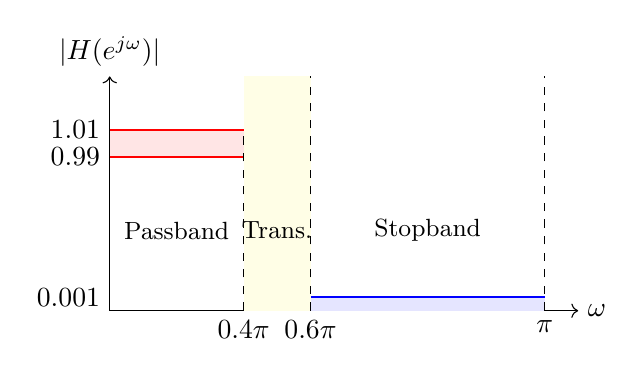
\begin{tikzpicture}[scale=0.85]
  \draw[->] (0,0) -- (7,0) node[right] {$\omega$};
  \draw[->] (0,0) -- (0,3. 5) node[above] {$|H(e^{j\omega})|$};
  
  % Passband
  \fill[red! 10] (0,2. 3) rectangle (2,2.7);
  \draw[thick, red] (0,2.7) -- (2,2.7);
  \draw[thick, red] (0,2.3) -- (2,2.3);
  \draw[dashed] (2,0) -- (2,2.7);
  \node[below] at (2,0) {$0.4\pi$};
  
  % Transition
  \fill[yellow!10] (2,0) rectangle (3,3.5);
  
  % Stopband
  \fill[blue!10] (3,0) rectangle (6. 5,0.2);
  \draw[thick, blue] (3,0. 2) -- (6.5,0.2);
  \draw[dashed] (3,0) -- (3,3.5);
  \node[below] at (3,0) {$0.6\pi$};
  \draw[dashed] (6.5,0) -- (6.5,3.5);
  \node[below] at (6. 5,0) {$\pi$};
  
  % Labels
  \node[left] at (0,2.7) {$1. 01$};
  \node[left] at (0,2.3) {$0.99$};
  \node[left] at (0,0. 2) {$0.001$};
  \node at (1,1.2) {\small Passband};
  \node at (2. 5,1.2) {\small Trans.};
  \node at (4. 75,1.2) {\small Stopband};
\end{tikzpicture}
\end{center}

\end{frame}

% %--------------------------------------------------
\begin{frame}{Filter Order Comparison}
\small

\textbf{For specifications:} $\omega_p = 0.4\pi$, $\omega_s = 0.6\pi$, $\delta_p = 0.01$, $\delta_s = 0.001$

\vspace{0.4cm}
\begin{center}
\begin{tabular}{lcc}
\hline
\textbf{Filter Type} & \textbf{Minimum Order} & \textbf{Zero Locations} \\
\hline
Butterworth & 14 & 14 zeros at $z=-1$ \\
Chebyshev I & 8 & 8 zeros at $z=-1$ \\
Chebyshev II & 8 & 8 zeros on unit circle \\
Elliptic & 6 & 6 zeros on unit circle \\
\hline
\end{tabular}
\end{center}

\vspace{0.4cm}
\textbf{Key Observations:}
\begin{itemize}
  \item Elliptic achieves lowest order (optimal)
  \item Butterworth requires $\sim 2\times$ the order of Chebyshev
  \item Chebyshev I simpler than II (all zeros at $z=-1$)
  \item Order directly impacts computational complexity
\end{itemize}

\end{frame}

%--------------------------------------------------
\section{Butterworth Filter}

\begin{frame}{Butterworth: Magnitude Response}
\small

\textbf{Order 14 Butterworth Filter}

\vspace{0.2cm}
\begin{center}
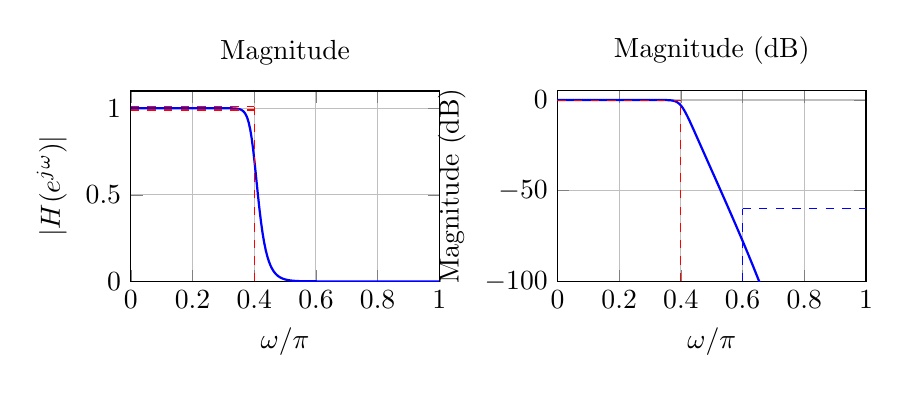
\begin{tikzpicture}
\begin{groupplot}[
    group style={
        group size=2 by 1,
        horizontal sep=1.5cm,
    },
    width=5.5cm,
    height=4cm,
]

% Linear magnitude
\nextgroupplot[
    xlabel={$\omega/\pi$},
    ylabel={$|H(e^{j\omega})|$},
    xmin=0, xmax=1,
    ymin=0, ymax=1. 1,
    grid=major,
    title={Magnitude},
]
\addplot[blue, thick, domain=0:1, samples=200] {1/sqrt(1 + (tan(x*90)/tan(36))^28)};
\draw[red, dashed] (axis cs:0,0.99) -- (axis cs:0. 4,0.99);
\draw[red, dashed] (axis cs:0,1.01) -- (axis cs:0.4,1.01);
\draw[red, dashed] (axis cs:0.4,0) -- (axis cs:0.4,1.01);
\draw[blue, dashed] (axis cs:0.6,0) -- (axis cs:0.6,0.001);
\draw[blue, dashed] (axis cs:0.6,0. 001) -- (axis cs:1,0.001);

% Log magnitude (dB)
\nextgroupplot[
    xlabel={$\omega/\pi$},
    ylabel={Magnitude (dB)},
    xmin=0, xmax=1,
    ymin=-100, ymax=5,
    grid=major,
    title={Magnitude (dB)},
]
\addplot[blue, thick, domain=0:1, samples=200] {20*log10(1/sqrt(1 + (tan(x*90)/tan(36))^28))};
\draw[red, dashed] (axis cs:0,-0.087) -- (axis cs:0. 4,-0.087);
\draw[red, dashed] (axis cs:0. 4,-100) -- (axis cs:0. 4,0);
\draw[blue, dashed] (axis cs:0. 6,-100) -- (axis cs:0. 6,-60);
\draw[blue, dashed] (axis cs:0. 6,-60) -- (axis cs:1,-60);

\end{groupplot}
\end{tikzpicture}
\end{center}

\vspace{0.1cm}
\textbf{Characteristics:}
\begin{itemize}
  \item Smooth, monotonic decrease (no ripple)
  \item Maximally flat at $\omega = 0$
  \item Gradual transition band roll-off
\end{itemize}

\end{frame}

%--------------------------------------------------

\begin{frame}{Butterworth: Pole-Zero Plot}
\small

\begin{columns}[T,onlytextwidth]
  \column{0.58\textwidth}
  \begin{center}
  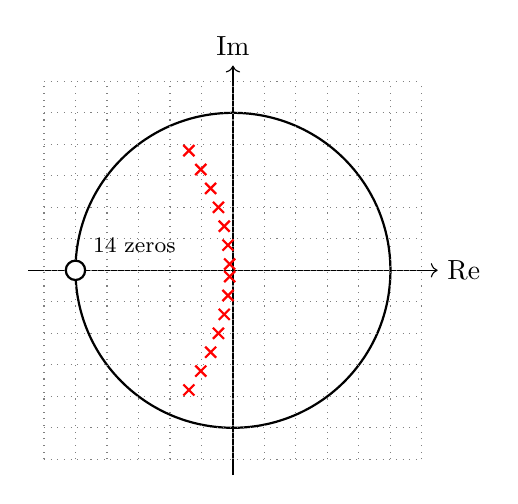
\begin{tikzpicture}[scale=2.0]
    % Unit circle
    \draw[thick] (0,0) circle (1);
    \draw[->] (-1.3,0) -- (1.3,0) node[right] {Re};
    \draw[->] (0,-1.3) -- (0,1.3) node[above] {Im};
    
    % Light grid for reference (optional)
    \draw[gray, dotted] (-1.2,-1.2) grid[step=0.2] (1.2,1.2);
    
    % 14 zeros at z = -1 (represented as a stacked marker with label)
    \node[circle, draw=black, fill=white, thick, minimum size=7pt, inner sep=0pt] at (-1,0) {};
    \node[above right] at (-0.95,0.05) {\footnotesize 14 zeros };
    
    % Poles: 7 conjugate pairs (N=14)
    % Place poles near a vertical line Re ~= 0 (small negative base), then add a y^2 bow to move them left for larger |Im|.
    % x = -base - bow_coeff * y^2
    \pgfmathsetmacro{\base}{0.02}    % base negative offset from Re=0
    \pgfmathsetmacro{\bow}{0.45}     % bow coefficient (controls how much they lean left)
    \foreach \k in {0,...,6} {
      \pgfmathsetmacro{\y}{0.04 + \k*0.12}               % imag: 0.04, 0.16, ..., up to ~0.76
      % compute x as small negative base plus bow to the left that grows with y^2
      \pgfmathsetmacro{\x}{- \base - \bow * (\y)^2}
      % draw pole as an "X" at (x,y) and its conjugate (x,-y)
      \draw[red, thick] (\x-0.035,\y-0.035) -- (\x+0.035,\y+0.035);
      \draw[red, thick] (\x-0.035,\y+0.035) -- (\x+0.035,\y-0.035);
      \draw[red, thick] (\x-0.035,-\y-0.035) -- (\x+0.035,-\y+0.035);
      \draw[red, thick] (\x-0.035,-\y+0.035) -- (\x+0.035,-\y-0.035);
    }
  \end{tikzpicture}
  \end{center}

  \column{0.42\textwidth}
  \textbf{Order 14 Butterworth Filter}

  \vspace{0.2cm}
  \textbf{Key Features:}
  \begin{itemize}
    \item Leftward bow increases with $|\mathrm{Im}|$ via a quadratic dependence on Im
    \item Poles placed at small negative Re and in conjugate pairs
    \item All poles kept inside the unit circle for stability
  \end{itemize}
\end{columns}

\end{frame}

%--------------------------------------------------
\section{Chebyshev Type I Filter}



\section{Chebyshev Type I Filter}

\begin{frame}{Chebyshev Type I: Magnitude Response}
\small

\textbf{Order \NText\ Chebyshev Type I Filter}

\vspace{0.2cm}
\begin{center}
\begin{tikzpicture}
  \begin{groupplot}[
      group style={
          group size=2 by 1,
          horizontal sep=1.5cm,
      },
      width=6cm,
      height=4cm,
  ]

  % Linear magnitude
  \nextgroupplot[
      xlabel={$\omega/\pi$},
      ylabel={$|H(e^{j\omega})|$},
      xmin=0, xmax=1,
      ymin=0, ymax=1.1,
      grid=major,
      title={Magnitude},
  ]
  % Passband: equiripple-like cosine visual model
  % Note: pgf math trig functions take degrees, so wrap angle with deg(...)
  \addplot[blue, thick, domain=0:\wpval, samples=600] {1 - \deltaval * cos(deg(2*pi * \Nval * x / \wpval))}; 
  % Stopband: monotonic decay (smooth polynomial rolloff)
  \addplot[blue, thick, domain=\wpval:1, samples=600] {1/(1 + 20000*(x-\wpval)^6)}; 
  % Passband ripple bounds and transition line
  \draw[red, dashed] (axis cs:0,{1-\deltaval}) -- (axis cs:\wpval,{1-\deltaval}); 
  \draw[red, dashed] (axis cs:0,{1+\deltaval}) -- (axis cs:\wpval,{1+\deltaval}); 
  \draw[red, dashed] (axis cs:\wpval,0) -- (axis cs:\wpval,1.05); 

  % Log magnitude (dB)
  \nextgroupplot[
      xlabel={$\omega/\pi$},
      ylabel={Magnitude (dB)},
      xmin=0, xmax=1,
      ymin=-100, ymax=5,
      grid=major,
      title={Magnitude (dB)},
  ]
  % Use max( , 1e-9) to avoid log of zero/negative
  \addplot[blue, thick, domain=0:\wpval, samples=600] {20*log10( max(1e-9, 1 - \deltaval * cos(deg(2*pi * \Nval * x / \wpval))))}; 
  \addplot[blue, thick, domain=\wpval:1, samples=600] {20*log10( max(1e-9, 1/(1 + 20000*(x-\wpval)^6)) )}; 
  % dB passband line and transition marker
  \draw[red, dashed] (axis cs:0,{20*log10(1-\deltaval)}) -- (axis cs:\wpval,{20*log10(1-\deltaval)}); 
  \draw[red, dashed] (axis cs:\wpval,-100) -- (axis cs:\wpval,5); 

  \end{groupplot}
\end{tikzpicture}
\end{center}

% \vspace{0.1cm}
\textbf{Characteristics:}
\begin{itemize}
  \item Equiripple behavior in the passband (visualized between $1-\DeltaText$ and $1+\DeltaText$)
  \item Monotonic, smoothly decaying stopband (no ripples)
\end{itemize}

\end{frame}


%------------------------

\begin{frame}{Chebyshev Type I: Pole-Zero Plot }
\small

\begin{columns}[T,onlytextwidth]
  \column{0.58\textwidth}
  \begin{center}
  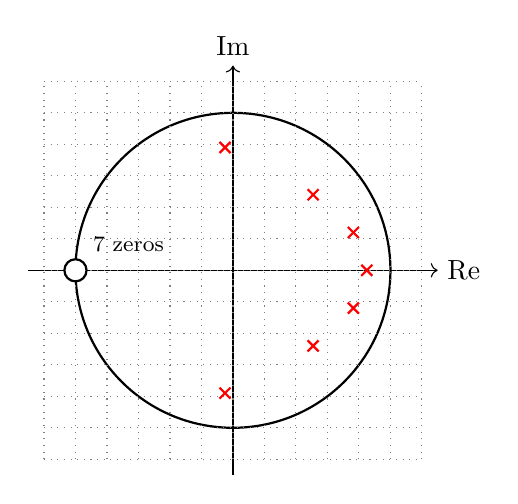
\begin{tikzpicture}[scale=2.0]
    % Parameters for quadratic curve x(y) = a - b y^2
    \pgfmathsetmacro{\a}{0.85}
    \pgfmathsetmacro{\b}{1.48}

    % Unit circle and axes
    \draw[thick] (0,0) circle (1);
    \draw[->] (-1.3,0) -- (1.3,0) node[right] {Re};
    \draw[->] (0,-1.3) -- (0,1.3) node[above] {Im};

    % Grid
    \draw[gray, dotted] (-1.2,-1.2) grid[step=0.2] (1.2,1.2);

    % 7 zeros at z = -1 (stacked visual marker)
    \node[circle, fill=white, draw=black, thick, minimum size=8pt, inner sep=0] at (-1,0) {};
    \node[above right] at (-0.95,0.06) {\footnotesize 7 zeros};

    % Real-axis pole (largest real component)
    \pgfmathsetmacro{\xreal}{\a} % = 0.85
    \draw[red, thick] (\xreal-0.035,-0.035) -- (\xreal+0.035,0.035);
    \draw[red, thick] (\xreal-0.035,0.035) -- (\xreal+0.035,-0.035);

    % Conjugate pairs
    \foreach \y in {0.24,0.48,0.78} {
      \pgfmathsetmacro{\xpole}{\a - \b*(\y*\y)}
      % Pole at (xpole, y)
      \draw[red, thick] (\xpole-0.035,\y-0.035) -- (\xpole+0.035,\y+0.035);
      \draw[red, thick] (\xpole-0.035,\y+0.035) -- (\xpole+0.035,\y-0.035);
      % Conjugate at (xpole, -y)
      \draw[red, thick] (\xpole-0.035,-\y-0.035) -- (\xpole+0.035,-\y+0.035);
      \draw[red, thick] (\xpole-0.035,-\y+0.035) -- (\xpole+0.035,-\y-0.035);
    }
  \end{tikzpicture}
  \end{center}

  \column{0.42\textwidth}
  \textbf{Key Features:}
  \begin{itemize}
    \item 7 zeros stacked at $z=-1$
    \item 7 poles lie on a smooth quadratic curve
    \item All poles remain inside the unit circle
  \end{itemize}
\end{columns}

\end{frame}

%--------------------------------------------------
\section{Chebyshev Type II Filter}


\begin{frame}{Chebyshev Type II: Magnitude Response}
\small

\textbf{Order \NText\ Chebyshev Type II Filter}

\vspace{0.2cm}
\begin{center}
\begin{tikzpicture}
  % local numeric for stopband edge (used only in this frame)
  \pgfmathsetmacro{\wsval}{0.6}    % normalized stopband edge (omega/pi)
  % number of stopband ripple cycles across the stopband
  \pgfmathsetmacro{\Nrip}{\Nval}   % reuse \Nval to set ripple density

  % passband / stopband baseline amplitudes
  \pgfmathsetmacro{\passAmp}{0.99}
  \pgfmathsetmacro{\stopAmp}{0.001}

  % Transition shaping parameters
  % transAlpha < 1 -> steeper onset right after \wpval
  \pgfmathsetmacro{\transAlpha}{0.45}    % smaller than 1 => steeper drop near wp
  % ripple growth exponent in transition: controls how quickly ripples grow
  \pgfmathsetmacro{\rippleGamma}{0.6}    % between 0 and 1 => ripple appears quickly near onset but still grows
  % We'll reuse the stopband ripple frequency (Nrip) so ripples are phase-aligned at ws
  % Transition ripple amplitude is chosen so that at x = ws the ripple matches the stopband ripple amplitude (0.8*stopAmp)
  % (stopband uses stopAmp*(1 + 0.8*cos(...)) so ripple amplitude at ws is 0.8*stopAmp).
  \pgfmathsetmacro{\transRippleAmp}{0.8 * \stopAmp}

  \begin{groupplot}[
      group style={
          group size=2 by 1,
          horizontal sep=1.5cm,
      },
      width=5.5cm,
      height=4cm,
  ]

  % Linear magnitude (split into three domains: passband, transition, stopband)
  \nextgroupplot[
      xlabel={$\omega/\pi$},
      ylabel={$|H(e^{j\omega})|$},
      xmin=0, xmax=1,
      ymin=0, ymax=1.1,
      grid=major,
      title={Magnitude},
  ]
  % Passband: smooth, monotonic envelope (no ripples)
  \addplot[blue, thick, domain=0:\wpval, samples=300] {
    \passAmp + \deltaval * sqrt( max(0, 1 - (x/\wpval)^2) )
  };
  % Transition band: shaped baseline (steeper at onset) + ripples that connect continuously to stopband ripples
  \addplot[blue, thick, domain=\wpval:\wsval, samples=500] {
    % normalized position in transition: 0..1
    % t = (x - wp) / (ws - wp)
    (% baseline: non-linear interpolation to make onset steeper
      \passAmp + (\stopAmp - \passAmp) * pow( (x - \wpval) / (\wsval - \wpval), \transAlpha )
    )
    % ripple: use same ripple phase/frequency as stopband (so cos() at ws = 1),
    % and grow its amplitude across the transition using envelope pow(t, rippleGamma)
    + \transRippleAmp * pow( max(0, (x - \wpval) / (\wsval - \wpval) ), \rippleGamma )
      * cos( deg( 2*pi * \Nrip * (x - \wsval) / (1 - \wsval) ) )
  };
  % Stopband: baseline with equiripple cosine oscillation (centered around ws..1)
  \addplot[blue, thick, domain=\wsval:1, samples=600] {
    \stopAmp * (1 + 0.8 * cos( deg( 2*pi * \Nrip * (x - \wsval) / (1 - \wsval) ) ) )
  };
  % passband spec line and transition markers
  \draw[red, dashed] (axis cs:0,\passAmp) -- (axis cs:\wpval,\passAmp);
  \draw[red, dashed] (axis cs:\wpval,0) -- (axis cs:\wpval,1.05);
  % stopband vertical marker at ws
  \draw[blue, dashed] (axis cs:\wsval,0) -- (axis cs:\wsval,0.02);
  % indicate transition endpoints with lighter vertical lines
  \draw[black, dashed] (axis cs:\wpval,0) -- (axis cs:\wpval,1.05);
  \draw[black, dashed] (axis cs:\wsval,0) -- (axis cs:\wsval,1.05);

  % Log magnitude (dB)
  \nextgroupplot[
      xlabel={$\omega/\pi$},
      ylabel={Magnitude (dB)},
      xmin=0, xmax=1,
      ymin=-120, ymax=5,
      grid=major,
      title={Magnitude (dB)},
  ]
  % passband (dB)
  \addplot[blue, thick, domain=0:\wpval, samples=300] {
    20*log10( max(1e-12, \passAmp + \deltaval * sqrt( max(0, 1 - (x/\wpval)^2) )) )
  };
  % transition band (dB) - same shaped baseline + ripples (ensures continuity of linear magnitude at ws)
  \addplot[blue, thick, domain=\wpval:\wsval, samples=500] {
    20*log10( max(1e-12,
      (% baseline same non-linear interpolation)
      \passAmp + (\stopAmp - \passAmp) * pow( (x - \wpval) / (\wsval - \wpval), \transAlpha )
      +
      % ripple term (same phase as stopband, grows via envelope)
      \transRippleAmp * pow( max(0, (x - \wpval) / (\wsval - \wpval) ), \rippleGamma )
        * cos( deg( 2*pi * \Nrip * (x - \wsval) / (1 - \wsval) ) )
    ))
  };
  % stopband (dB)
  \addplot[blue, thick, domain=\wsval:1, samples=600] {
    20*log10( max(1e-12, \stopAmp * (1 + 0.8 * cos( deg( 2*pi * \Nrip * (x - \wsval) / (1 - \wsval) ) ) ) ) )
  };
  % vertical markers: passband/transition and stopband region
  \draw[red, dashed] (axis cs:\wpval,-120) -- (axis cs:\wpval,5);
  \draw[blue, dashed] (axis cs:\wsval,-120) -- (axis cs:\wsval,5);

  \end{groupplot}
\end{tikzpicture}
\end{center}

\vspace{0.1cm}
\textbf{Characteristics:}
\begin{itemize}
  \item Monotonic in passband (smooth like Butterworth)
  \item Equiripple in stopband (oscillates around the stopband baseline)
  \item Stopband nulls originate from zeros placed on or near the unit circle
\end{itemize}

\end{frame}



%--------------------------------------------------



\begin{frame}{Chebyshev Type II: Pole-Zero Plot}
\small

\begin{columns}[T,onlytextwidth]
  \column{0.58\textwidth}
  \begin{center}
  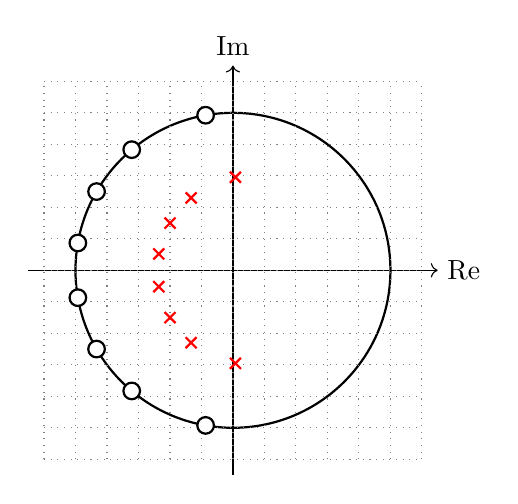
\begin{tikzpicture}[scale=2.0]
    % Unit circle and axes
    \draw[thick] (0,0) circle (1);
    \draw[->] (-1.3,0) -- (1.3,0) node[right] {Re};
    \draw[->] (0,-1.3) -- (0,1.3) node[above] {Im};

    % Light grid
    \draw[gray, dotted] (-1.2,-1.2) grid[step=0.2] (1.2,1.2);

    % Angles for zeros/poles (upper half angles, and their negatives for conjugates)
    \def\angles{100,130,150,170,-100,-130,-150,-170}

    % Draw zeros on unit circle (conjugate pairs)
    \foreach \angle in \angles {
      \node[circle, fill=white, draw=black, thick, minimum size=6pt, inner sep=0] at (\angle:1) {};
    }

    % Poles: radius 0.60, shifted right by +0.12 (conjugate pairs)
    \pgfmathsetmacro{\poleRadius}{0.60}
    \pgfmathsetmacro{\dx}{0.12}

    \foreach \angle in \angles {
      \pgfmathsetmacro{\xbase}{\poleRadius*cos(\angle)}
      \pgfmathsetmacro{\ybase}{\poleRadius*sin(\angle)}
      \pgfmathsetmacro{\x}{\xbase + \dx}
      % red X for pole
      \draw[red, thick] (\x-0.035,\ybase-0.035) -- (\x+0.035,\ybase+0.035);
      \draw[red, thick] (\x-0.035,\ybase+0.035) -- (\x+0.035,\ybase-0.035);
    }
  \end{tikzpicture}
  \end{center}

  \column{0.42\textwidth}
  \textbf{Order 8 Chebyshev Type II Filter}

  \vspace{0.2cm}
  \textbf{Key Features:}
  \begin{itemize}
    \item 8 zeros on the unit circle arranged as conjugate pairs
    \item 8 poles placed inside the unit circle 
  \end{itemize}
\end{columns}

\end{frame}



%--------------------------------------------------
\section{Elliptic Filter}




\begin{frame}{Elliptic: Magnitude Response}
\small

\textbf{Order 6 Elliptic Filter (Optimal)}

% \vspace{0.2cm}
\begin{center}
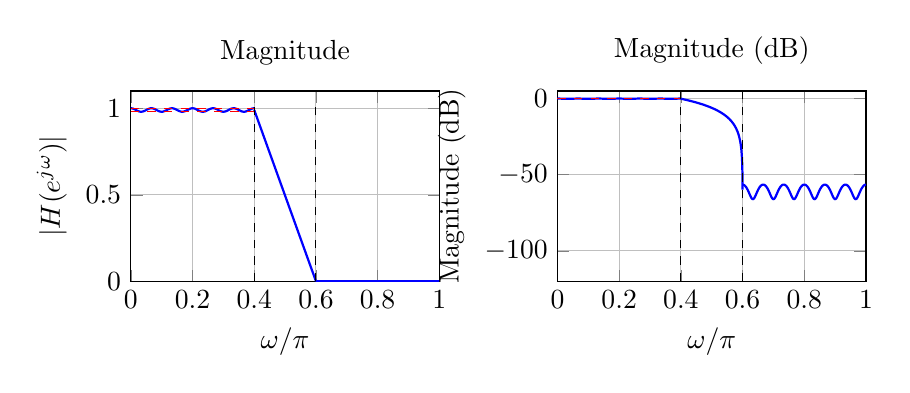
\begin{tikzpicture}
% edges
\pgfmathsetmacro{\wpval}{0.4}   % passband edge (omega/pi)
\pgfmathsetmacro{\wsval}{0.6}   % stopband edge (omega/pi)

% ripple / baseline parameters
\pgfmathsetmacro{\passCenter}{0.99}    % passband center amplitude (linear)
\pgfmathsetmacro{\passAmp}{0.01}       % passband ripple amplitude (linear)
\pgfmathsetmacro{\passCycles}{6}       % number of ripple cycles across passband

\pgfmathsetmacro{\stopCenter}{0.001}   % stopband baseline amplitude (linear)
\pgfmathsetmacro{\stopDepth}{0.5}      % relative depth of stopband ripple (0..1)
\pgfmathsetmacro{\stopCycles}{6}       % number of ripple cycles across stopband

% precompute numeric envelope and dB helpers to avoid inline math inside coordinates
\pgfmathsetmacro{\passHigh}{\passCenter + \passAmp}   % numeric
\pgfmathsetmacro{\passLow}{\passCenter - \passAmp}    % numeric
\pgfmathsetmacro{\passHighdB}{20*log10(max(1e-12,\passHigh))}
\pgfmathsetmacro{\passLowdB}{20*log10(max(1e-12,\passLow))}
\pgfmathsetmacro{\stopPeak}{\stopCenter*(1+\stopDepth)}
\pgfmathsetmacro{\stopPeakdB}{20*log10(max(1e-12,\stopPeak))}

\begin{groupplot}[
    group style={
        group size=2 by 1,
        horizontal sep=1.5cm,
    },
    width=5.5cm,
    height=4cm,
]

% Linear magnitude (passband: equiripple; transition: smooth; stopband: equiripple)
\nextgroupplot[
    xlabel={$\omega/\pi$},
    ylabel={$|H(e^{j\omega})|$},
    xmin=0, xmax=1,
    ymin=0, ymax=1.1,
    grid=major,
    title={Magnitude},
]
% passband: equiripple symmetric about passCenter
\addplot[blue, thick, domain=0:\wpval, samples=600] {
  \passCenter + \passAmp * cos( deg( 2*pi * \passCycles * x / \wpval ) )
};
% transition: smooth monotonic drop (no ripples)
\addplot[blue, thick, domain=\wpval:\wsval, samples=400] {
  \passCenter + (\stopCenter - \passCenter) * ((x - \wpval)/(\wsval - \wpval))
};
% stopband: equiripple around stopCenter (relative ripple depth)
\addplot[blue, thick, domain=\wsval:1, samples=600] {
  \stopCenter * ( 1 + \stopDepth * cos( deg( 2*pi * \stopCycles * (x - \wsval) / (1 - \wsval) ) ) )
};
% passband ripple envelope lines (use precomputed numeric macros)
\draw[red, dashed] (axis cs:0,\passHigh) -- (axis cs:\wpval,\passHigh);
\draw[red, dashed] (axis cs:0,\passLow) -- (axis cs:\wpval,\passLow);
% passband / stopband edge markers
\draw[black, dashed] (axis cs:\wpval,0) -- (axis cs:\wpval,1.05);
\draw[black, dashed] (axis cs:\wsval,0) -- (axis cs:\wsval,1.05);

% Log magnitude (dB)
\nextgroupplot[
    xlabel={$\omega/\pi$},
    ylabel={Magnitude (dB)},
    xmin=0, xmax=1,
    ymin=-120, ymax=5,
    grid=major,
    title={Magnitude (dB)},
]
% passband (dB) - convert safely with max()
\addplot[blue, thick, domain=0:\wpval, samples=600] {
  20*log10( max(1e-12, \passCenter + \passAmp * cos( deg( 2*pi * \passCycles * x / \wpval ) ) ) )
};
% transition (dB)
\addplot[blue, thick, domain=\wpval:\wsval, samples=400] {
  20*log10( max(1e-12, \passCenter + (\stopCenter - \passCenter) * ((x - \wpval)/(\wsval - \wpval)) ) )
};
% stopband (dB)
\addplot[blue, thick, domain=\wsval:1, samples=600] {
  20*log10( max(1e-12, \stopCenter * ( 1 + \stopDepth * cos( deg( 2*pi * \stopCycles * (x - \wsval) / (1 - \wsval) ) ) ) ) )
};
% passband ripple envelope in dB (peaks) using precomputed numeric macros
\draw[red, dashed] (axis cs:0,\passHighdB) -- (axis cs:\wpval,\passHighdB);
\draw[red, dashed] (axis cs:0,\passLowdB) -- (axis cs:\wpval,\passLowdB);
% region markers
\draw[black, dashed] (axis cs:\wpval,-120) -- (axis cs:\wpval,5);
\draw[black, dashed] (axis cs:\wsval,-120) -- (axis cs:\wsval,5);

\end{groupplot}
\end{tikzpicture}
\end{center}

% \vspace{0.1cm}
\textbf{Characteristics:}
\begin{itemize}
  \item Equiripple in both passband and stopband 
  \item Smooth finite transition band 
  \item Sharp transition and strong stopband attenuation typical of elliptic filters
\end{itemize}

\end{frame}



%--------------------------------------------------


\begin{frame}{Elliptic: Pole-Zero Plot}
\small

\begin{columns}[T,onlytextwidth]
  \column{0.58\textwidth}
  \begin{center}
  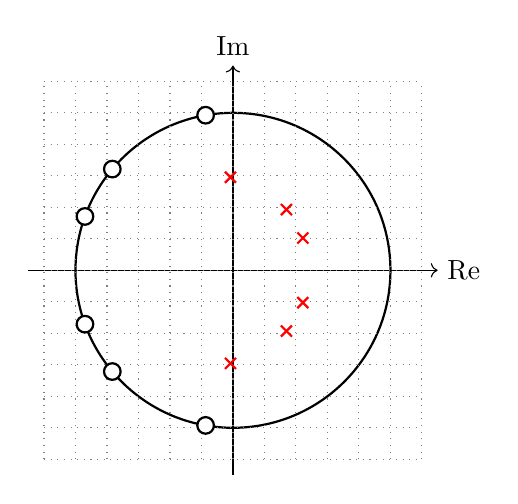
\begin{tikzpicture}[scale=2.0]
    % Unit circle and axes
    \draw[thick] (0,0) circle (1);
    \draw[->] (-1.3,0) -- (1.3,0) node[right] {Re};
    \draw[->] (0,-1.3) -- (0,1.3) node[above] {Im};

    % Light grid
    \draw[gray, dotted] (-1.2,-1.2) grid[step=0.2] (1.2,1.2);

    % Angles for zeros (placed similarly to Chebyshev Type II but only 6)
    \def\angles{100,140,160,-100,-140,-160}

    % Draw zeros on unit circle (conjugate pairs)
    \foreach \angle in \angles {
      \node[circle, fill=white, draw=black, thick, minimum size=6pt, inner sep=0] at (\angle:1) {};
    }

    % Chebyshev-II pole parameters (radius 0.60, shifted right by +0.12)
    \pgfmathsetmacro{\poleRadius}{0.60}
    \pgfmathsetmacro{\dx}{0.12}

    % For the elliptic filter reflect those Chebyshev-II poles across the y-axis:
    % x_ellip = - (poleRadius*cos(angle) + dx)
    \foreach \angle in \angles {
      \pgfmathsetmacro{\xbase}{\poleRadius*cos(\angle)}
      \pgfmathsetmacro{\ybase}{\poleRadius*sin(\angle)}
      \pgfmathsetmacro{\x}{- (\xbase + \dx)} % reflection across y-axis
      % draw red "X" for reflected pole
      \draw[red, thick] (\x-0.035,\ybase-0.035) -- (\x+0.035,\ybase+0.035);
      \draw[red, thick] (\x-0.035,\ybase+0.035) -- (\x+0.035,\ybase-0.035);
    }
  \end{tikzpicture}
  \end{center}

  \column{0.42\textwidth}
  \textbf{Order 6 Elliptic Filter}

  \vspace{0.2cm}
  \textbf{Key Features:}
  \begin{itemize}
    \item 6 zeros on the unit circle arranged as conjugate pairs (placed similarly to the Chebyshev Type II zeros)
    \item 6 poles in complex conjugate pairs and within unit circle
  \end{itemize}
\end{columns}

\end{frame}


%--------------------------------------------------
\section{Conclusion}

\begin{frame}{Key Takeaways}
\small

\textbf{Visual Summary:}

\vspace{0.3cm}
\begin{center}
\small
\begin{tabular}{lccc}
\hline
\textbf{Type} & \textbf{Order} & \textbf{Passband} & \textbf{Stopband} \\
\hline
Butterworth & 14 & Monotonic & Monotonic \\
Chebyshev I & 8 & Equiripple & Monotonic \\
Chebyshev II & 8 & Monotonic & Equiripple \\
Elliptic & 6 & Equiripple & Equiripple \\
\hline
\end{tabular}
\end{center}

\vspace{0.3cm}
\textbf{Selection Guide:}
\begin{itemize}
  \item \textbf{Minimize order/cost? } $\rightarrow$ Elliptic
  \item \textbf{Smooth response?} $\rightarrow$ Butterworth
  \item \textbf{Balance efficiency \& simplicity?} $\rightarrow$ Chebyshev I
  \item \textbf{Smooth passband, lower order?} $\rightarrow$ Chebyshev II
\end{itemize}

\vspace{0.3cm}
\textbf{All zeros at $z=-1$:} Butterworth, Chebyshev I (simpler implementation)

\textbf{Zeros on unit circle:} Chebyshev II, Elliptic (stopband nulls, causes stopband ripples)

\end{frame}





\end{document}

